% ============================================================
% CHAPTER 3 — DATASETS AND EXPERIMENTAL SETUP
% Final M.Tech Thesis: Uncertainty-Aware Triage Learning for
% Medical Image Diagnosis: A Human-AI Collaborative Framework
% ============================================================

\chapter{DATASETS AND EXPERIMENTAL SETUP}

\section{MedMNIST Benchmark Overview}

The MedMNIST benchmark collection~\cite{yang2021medmnist} provides a standardised suite of biomedical image classification datasets in a unified, lightweight format. Each dataset is pre-processed to a resolution of 28$\times$28 pixels per image, supplied with fixed train-validation-test splits, and accompanied by canonical evaluation metrics, enabling direct reproducibility and cross-study comparison without dataset-specific preprocessing decisions. The benchmark spans multiple imaging modalities, anatomical regions, and clinical tasks, making it well-suited for evaluating the generalisability of machine learning frameworks across diverse medical imaging conditions.

Three datasets from the MedMNIST v2 collection are employed in this thesis: PathMNIST for histopathological tissue classification, ChestMNIST for multi-label chest radiograph disease detection, and DermaMNIST for dermatoscopic skin lesion classification. These three were selected to ensure diversity along three key axes: imaging modality (optical microscopy, X-ray, and dermoscopy), classification task structure (single-label multi-class versus multi-label binary), and dataset scale (small, medium, and large). Table~\ref{tab:medmnist_overview} summarises the key characteristics of each dataset; Figure~\ref{fig:dataset_overview} visualises the class distribution within each.

\begin{table}[h]
\footnotesize
\centering
\caption{Summary of MedMNIST Datasets Used in This Work}
\label{tab:medmnist_overview}
\begin{tabular}{lcccccc}
\toprule
\textbf{Dataset} & \textbf{Modality} & \textbf{Total N} & \textbf{Train} & \textbf{Val} & \textbf{Test} & \textbf{Classes} \\
\midrule
PathMNIST   & Histopathology (RGB)    & 89,996  & 62,997 & 13,499 & 13,500 & 9 (single-label) \\
ChestMNIST  & Chest X-ray (greyscale) & 112,120 & 78,484 & 16,818 & 16,818 & 14 (multi-label) \\
DermaMNIST  & Dermatoscopy (RGB)      & 10,015  &  7,010 &  1,503 &  1,502 & 7 (single-label) \\
\bottomrule
\end{tabular}
\end{table}

\begin{figure}[h]
\centering
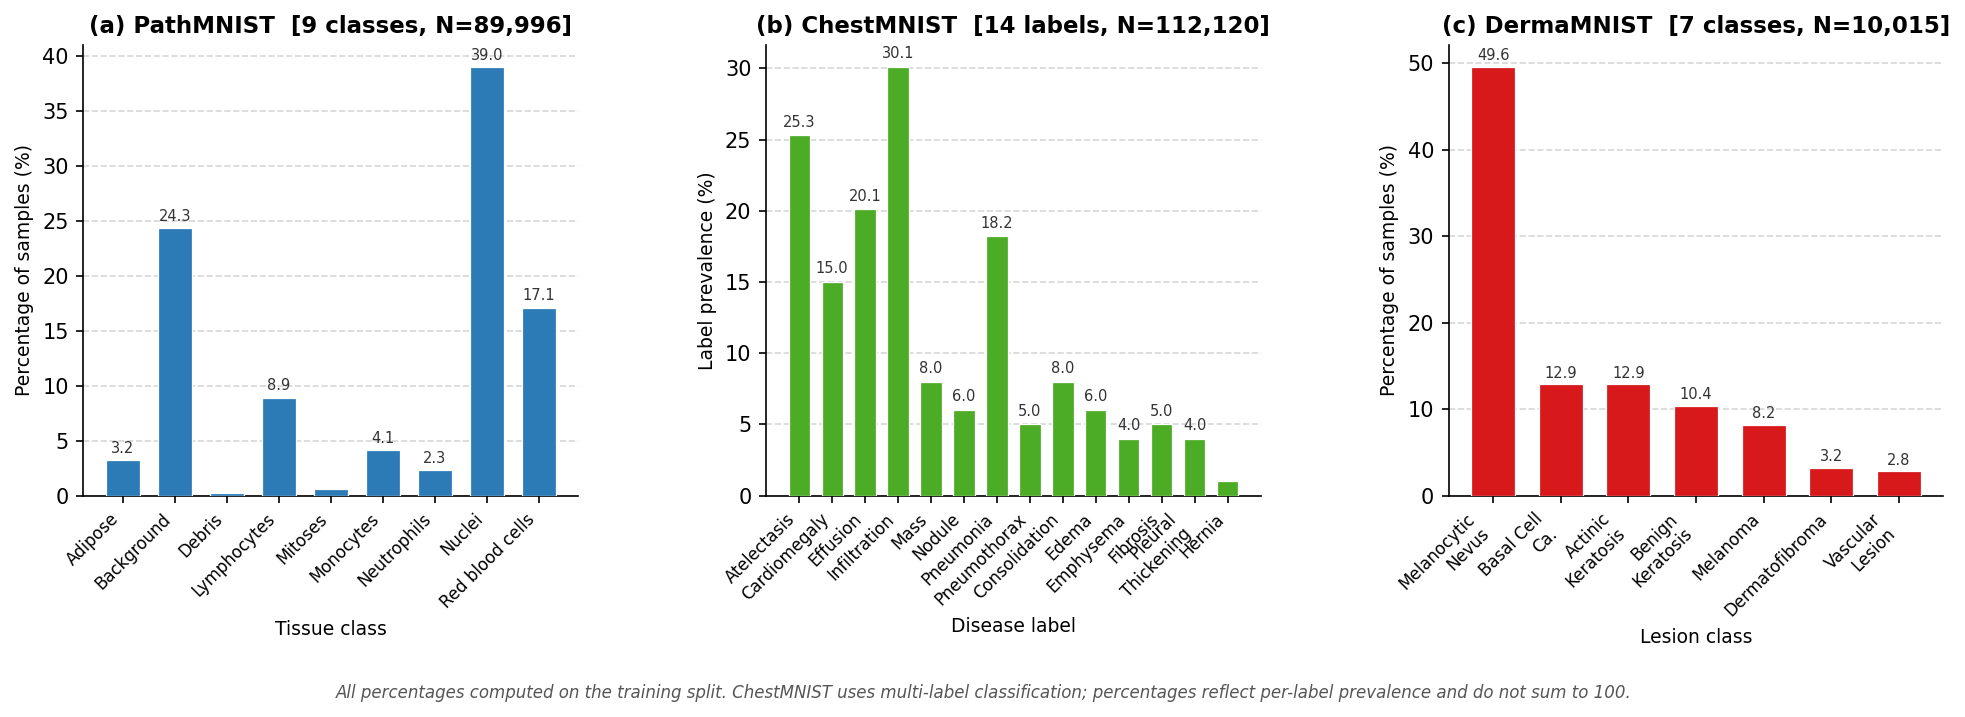
\includegraphics[width=\textwidth]{chapters/fig_dataset_overview.png}
\caption{Class distribution across the three MedMNIST datasets. (a) PathMNIST exhibits extreme imbalance (195:1), dominated by nuclei and background tissue. (b) ChestMNIST label prevalences vary by over 30$\times$, with Infiltration the most common and Hernia the rarest. (c) DermaMNIST is dominated by Melanocytic Nevus at 49.6\%, with Vascular Lesion and Dermatofibroma collectively representing under 6\% of samples.}
\label{fig:dataset_overview}
\end{figure}

All images are loaded as uint8 arrays in the range $[0, 255]$ and subsequently normalised during preprocessing. Greyscale ChestMNIST images are replicated across three channels to enable use of RGB-pretrained architectures without architectural modification. The standard MedMNIST splits are used throughout without modification, ensuring comparability with published baselines.

\section{PathMNIST — Histopathology Classification}

\subsection{Dataset Provenance and Clinical Context}

PathMNIST is derived from the colorectal cancer histopathology dataset introduced by Kather et al.~\cite{kather2019predicting}, which contains 100,000 non-overlapping image patches extracted from haematoxylin-and-eosin (H\&E) stained whole-slide images of human colorectal cancer and normal tissue. The task is to classify each 224$\times$224 pixel patch into one of nine tissue types, which are then downsampled to 28$\times$28 pixels for the MedMNIST benchmark. Accurate classification of tissue microenvironment components is clinically relevant for tumour microenvironment characterisation, treatment response prediction, and identification of microsatellite instability~\cite{kather2019predicting}.

\subsection{Class Definitions and Distribution}

The nine tissue classes represent distinct histological entities encountered in colorectal resection specimens. Table~\ref{tab:pathmnist_classes} enumerates the classes, their approximate training set frequencies, and their clinical significance.

\begin{table}[h]
\footnotesize
\centering
\caption{PathMNIST Class Definitions and Training Set Distribution}
\label{tab:pathmnist_classes}
\begin{tabular}{clcc}
\toprule
\textbf{Index} & \textbf{Class} & \textbf{Train count} & \textbf{Train \%} \\
\midrule
0 & Adipose (fat tissue)    & 2,016  & 3.2\%  \\
1 & Background              & 15,286 & 24.3\% \\
2 & Debris                  & 126    & 0.2\%  \\
3 & Lymphocytes             & 5,603  & 8.9\%  \\
4 & Mitoses                 & 378    & 0.6\%  \\
5 & Monocytes               & 2,583  & 4.1\%  \\
6 & Neutrophils             & 1,449  & 2.3\%  \\
7 & Nuclei (tumour epithelium) & 24,569 & 39.0\% \\
8 & Red blood cells         & 10,773 & 17.1\% \\
\midrule
\multicolumn{2}{l}{\textbf{Imbalance ratio (Nuclei:Debris)}} & \multicolumn{2}{c}{195:1} \\
\bottomrule
\end{tabular}
\end{table}

The dataset exhibits a severe imbalance ratio of 195:1 between the dominant class (Nuclei, 39\%) and the rarest class (Debris, 0.2\%). This extreme skew motivates the use of class-weighted loss functions and balanced accuracy as a complementary evaluation metric to overall accuracy. The seven test-set samples used in the main triage analysis number 7,180, drawn from the canonical test split.

\subsection{Known Challenges}

At 28$\times$28 pixel resolution, fine-grained cellular morphology—such as nuclear pleomorphism, mitotic figure detail, and glandular architecture—is largely unresolvable. Classes such as Mitoses (0.6\%) and Debris (0.2\%) present both extreme rarity and limited visual distinctiveness at this resolution, making them the primary sources of classification error. Inter-class visual similarity is highest between Monocytes and Lymphocytes, and between Neutrophils and other small-cell types, consistent with the confusion patterns observed in the trained model.

\section{ChestMNIST — Chest X-ray Multi-label Classification}

\subsection{Dataset Provenance and Clinical Context}

ChestMNIST is derived from the NIH ChestX-ray14 dataset~\cite{wang2017chestx}, which comprises 112,120 frontal-view chest radiographs from 30,805 unique patients collected at the NIH Clinical Center. Each image is annotated with up to 14 binary disease labels extracted from radiology reports via natural language processing. The dataset covers a broad spectrum of thoracic pathology including structural abnormalities (Atelectasis, Cardiomegaly, Effusion, Pneumothorax), infiltrative processes (Infiltration, Consolidation, Edema, Pneumonia), and chronic interstitial disease (Emphysema, Fibrosis, Pleural Thickening). Chest radiograph interpretation is a high-volume, high-stakes task in clinical practice; errors in detecting Pneumothorax or Pneumonia can have immediate life-threatening consequences.

\subsection{Class Definitions, Label Structure, and Distribution}

Unlike PathMNIST, ChestMNIST employs a multi-label formulation: each image may carry zero, one, or multiple simultaneous disease labels, reflecting the clinical reality that patients frequently present with co-morbid thoracic pathology. Table~\ref{tab:chestmnist_classes} lists all 14 disease labels with their approximate per-label prevalence in the training split.

\begin{table}[h]
\footnotesize
\centering
\caption{ChestMNIST Disease Labels and Training Set Prevalence}
\label{tab:chestmnist_classes}
\begin{tabular}{clcc}
\toprule
\textbf{Index} & \textbf{Disease} & \textbf{Prevalence (\%)} & \textbf{Clinical Priority} \\
\midrule
0  & Atelectasis       & 25.3\% & Moderate \\
1  & Cardiomegaly      & 15.0\% & High     \\
2  & Effusion          & 20.1\% & High     \\
3  & Infiltration      & 30.1\% & Moderate \\
4  & Mass              & 8.0\%  & High     \\
5  & Nodule            & 6.0\%  & High     \\
6  & Pneumonia         & 18.2\% & Critical \\
7  & Pneumothorax      & 5.0\%  & Critical \\
8  & Consolidation     & 8.0\%  & High     \\
9  & Edema             & 6.0\%  & High     \\
10 & Emphysema         & 4.0\%  & Moderate \\
11 & Fibrosis          & 5.0\%  & Moderate \\
12 & Pleural Thickening& 4.0\%  & Low      \\
13 & Hernia            & 1.0\%  & Low      \\
\midrule
\multicolumn{2}{l}{\textbf{Imbalance ratio (Infiltration:Hernia)}} & \multicolumn{2}{c}{$\approx$30:1} \\
\bottomrule
\end{tabular}
\end{table}

The multi-label structure means that evaluation via standard multi-class accuracy is inappropriate; per-label AUC (area under the ROC curve) and mean AUC across all 14 labels are the canonical metrics for this dataset. Approximately 10\% of samples carry a single label, 30\% carry two, 35\% carry three, and 25\% carry four or more, reflecting realistic clinical comorbidity patterns.

\subsection{Known Challenges}

The NLP-derived labels in ChestX-ray14 are known to carry non-trivial noise~\cite{rajpurkar2017chexnet}: report language ambiguities, negation errors, and label inheritance from prior studies introduce label noise estimated at 5--10\% for some categories. At 28$\times$28 resolution, subtle findings such as small pulmonary nodules, early consolidation, and pleural thickening are difficult or impossible to detect visually. The greyscale single-channel nature of chest radiographs removes colour as a discriminative cue. These challenges collectively make ChestMNIST the most difficult of the three datasets evaluated in this work.

\section{DermaMNIST — Dermatoscopy Classification}

\subsection{Dataset Provenance and Clinical Context}

DermaMNIST is sourced from the HAM10000 (Human Against Machine with 10,000 training images) dataset~\cite{tschandl2018ham10000}, a large collection of dermatoscopic images compiled from multiple clinical centres across Austria and Australia. The dataset was assembled specifically to train and evaluate machine learning models for automated melanoma detection and differential diagnosis of common pigmented skin lesions. Accurate classification is clinically critical: Melanoma, if detected at an early stage, has a five-year survival rate exceeding 95\%; late-stage diagnosis reduces this to below 20\%. The seven-class formulation covers the most common dermatological entities encountered in clinical practice.

\subsection{Class Definitions and Distribution}

Table~\ref{tab:dermamnist_classes} lists the seven classes with their training set frequencies and cancer status.

\begin{table}[h]
\footnotesize
\centering
\caption{DermaMNIST Class Definitions and Training Set Distribution}
\label{tab:dermamnist_classes}
\begin{tabular}{clccc}
\toprule
\textbf{Index} & \textbf{Class} & \textbf{Train count} & \textbf{Train \%} & \textbf{Malignant?} \\
\midrule
0 & Melanoma               & 575  & 8.2\%  & Yes (high risk) \\
1 & Melanocytic Nevus      & 3,476 & 49.6\% & No              \\
2 & Basal Cell Carcinoma   & 904  & 12.9\% & Yes             \\
3 & Actinic Keratosis      & 904  & 12.9\% & Precancerous    \\
4 & Benign Keratosis       & 729  & 10.4\% & No              \\
5 & Dermatofibroma         & 224  & 3.2\%  & No              \\
6 & Vascular Lesion        & 196  & 2.8\%  & No              \\
\midrule
\multicolumn{2}{l}{\textbf{Imbalance ratio (Melanocytic Nevus:Vascular Lesion)}} & \multicolumn{2}{c}{18:1} \\
\multicolumn{2}{l}{\textbf{Cancer/precancer prevalence}} & \multicolumn{2}{c}{34.0\%} \\
\bottomrule
\end{tabular}
\end{table}

Although the imbalance ratio (18:1) is less extreme than PathMNIST, the clinical asymmetry of errors is higher: misclassifying a Melanoma as a Melanocytic Nevus (false negative) can result in delayed treatment with life-threatening consequences, while the reverse error (unnecessary biopsy) imposes procedural burden but no mortality risk. This asymmetry motivates the use of per-class recall and cancer-class sensitivity as additional evaluation metrics.

\subsection{Known Challenges}

DermaMNIST is the smallest of the three datasets (10,015 total samples), increasing the risk of overfitting and making reliable uncertainty estimation more challenging due to the limited calibration set size. The fine-grained colour and texture features that distinguish, for example, Melanoma from Melanocytic Nevus—irregular dermoscopic patterns, atypical vascular structures, and specific colour gradients—are substantially degraded at 28$\times$28 resolution. Confusions between Actinic Keratosis and Basal Cell Carcinoma, and between Dermatofibroma and Melanocytic Nevus, are expected given their overlapping morphological appearances even at clinical resolution.

\section{Data Preprocessing and Augmentation}

\subsection{Preprocessing Pipeline}

A unified preprocessing pipeline is applied to all three datasets, with minor dataset-specific adjustments. The pipeline proceeds in the following steps:

\begin{enumerate}
    \item \textbf{Type conversion:} Raw uint8 images in $[0, 255]$ are cast to float32 and divided by 255 to yield values in $[0.0, 1.0]$.
    \item \textbf{Channel replication (ChestMNIST only):} Single-channel greyscale images are replicated across three channels to produce tensors of shape $(3, H, W)$, enabling use of ImageNet-pretrained RGB architectures without modification.
    \item \textbf{ImageNet standardisation:} All images are standardised per-channel using ImageNet statistics: $\boldsymbol{\mu} = [0.485, 0.456, 0.406]$ and $\boldsymbol{\sigma} = [0.229, 0.224, 0.225]$. For the greyscale-replicated ChestMNIST images, the three channels are identical prior to this step, and the per-channel mean and variance shift them to be compatible with the expected activation statistics of pretrained convolutional feature extractors.
    \item \textbf{Tensor formatting:} Images are transposed from HWC (height $\times$ width $\times$ channels) to CHW (channels $\times$ height $\times$ width) as required by PyTorch.
\end{enumerate}

\subsection{Data Augmentation}

Augmentation is applied to the training split only, with separate policies per dataset reflecting their distinct clinical characteristics. No augmentation is applied at validation or test time.

\subsubsection{PathMNIST Augmentation (Standard Policy)}

Histopathology images do not have a canonical orientation; tissue sections can be captured at arbitrary rotation angles and are rotationally symmetric in the diagnostic context. The following augmentations are applied:

\begin{itemize}
    \item Random horizontal flip with probability 0.5
    \item Random vertical flip with probability 0.5
    \item Random rotation in the range $[-15°, +15°]$
    \item Colour jitter: brightness $\pm 20\%$, contrast $\pm 20\%$, saturation $\pm 20\%$, hue $\pm 5\%$
\end{itemize}

\subsubsection{ChestMNIST Augmentation (Conservative Policy)}

Chest radiographs have an inherent anatomical orientation; vertical flipping would produce anatomically impossible images. Augmentation is therefore more conservative:

\begin{itemize}
    \item Random horizontal flip with probability 0.3 (mild; some X-ray views permit this)
    \item No vertical flip
    \item Random rotation in the range $[-10°, +10°]$
    \item Brightness and contrast jitter $\pm 10\%$ only; no saturation or hue augmentation
    \item Random Gaussian blur with $\sigma \in [0.1, 0.5]$, probability 0.1
\end{itemize}

\subsubsection{DermaMNIST Augmentation (Colour-Preserving Policy)}

Dermoscopic classification relies heavily on colour information (melanin distribution, vascular patterns). Aggressive colour augmentation may destroy diagnostically relevant features:

\begin{itemize}
    \item Random horizontal and vertical flip with probability 0.5 each
    \item Random rotation in the range $[-20°, +20°]$
    \item Brightness $\pm 10\%$, contrast $\pm 10\%$, saturation $\pm 10\%$ jitter
    \item Hue jitter limited to $\pm 5\%$ to preserve colour diagnostics
    \item No elastic deformation (lesion shape is diagnostically informative)
\end{itemize}

\subsection{Class Imbalance Handling}

In addition to augmentation, class imbalance is addressed at the loss function level during training. Per-class weights are computed as $w_c = n / (C \cdot n_c)$, where $n$ is the total number of training samples, $C$ is the number of classes, and $n_c$ is the per-class sample count. These weights up-weight minority classes in the cross-entropy loss without oversampling, avoiding the memorisation risk associated with instance duplication. For ChestMNIST, the weighting is applied independently per label in the binary cross-entropy objective.

\section{Evaluation Metrics and Protocol}

\subsection{Classification Metrics}

The following classification metrics are computed on the held-out test split for each dataset:

\begin{itemize}
    \item \textbf{Accuracy:} $\text{Acc} = N^{-1}\sum_{i=1}^N \mathbb{I}(\hat{y}_i = y_i)$. Reported for PathMNIST and DermaMNIST (single-label tasks).
    \item \textbf{Balanced accuracy:} Macro-average of per-class recall, $\text{BAcc} = C^{-1}\sum_{c=1}^C \text{Recall}_c$. Accounts for class imbalance by giving equal weight to each class regardless of frequency.
    \item \textbf{Precision, recall, F1 score:} Macro-averaged across classes. F1 is the harmonic mean of precision and recall, providing a single scalar that balances both.
    \item \textbf{Mean AUC (ChestMNIST):} Per-label area under the receiver operating characteristic curve, averaged across all 14 labels. This is the canonical metric for ChestMNIST evaluation.
    \item \textbf{Cross-entropy loss:} Evaluated on the test split as a measure of probability calibration quality prior to post-hoc calibration.
\end{itemize}

\subsection{Uncertainty Quality Metrics}

Uncertainty estimation quality is assessed via the following metrics:

\begin{itemize}
    \item \textbf{Point-biserial correlation ($r_{pb}$):} Correlation between scalar uncertainty scores and the binary error indicator ($1$ if $\hat{y}_i \neq y_i$, $0$ otherwise). Directly quantifies the utility of uncertainty as a predictor of errors.
    \item \textbf{Spearman rank correlation ($\rho_s$):} Non-parametric rank correlation between uncertainty and error indicator; does not assume linearity.
    \item \textbf{AUROC (uncertainty as error predictor):} Area under the ROC curve treating high uncertainty as a positive signal for prediction error. An AUROC of 1.0 indicates perfect error detection; 0.5 indicates random prediction.
\end{itemize}

\subsection{Calibration Metrics}

\begin{itemize}
    \item \textbf{Expected Calibration Error (ECE):} Computed with $B=15$ equal-width confidence bins. $\text{ECE} = \sum_b (|B_b|/n)\,|\text{acc}(B_b) - \text{conf}(B_b)|$.
    \item \textbf{Maximum Calibration Error (MCE):} $\text{MCE} = \max_b |\text{acc}(B_b) - \text{conf}(B_b)|$. Measures worst-case bin-level miscalibration.
    \item \textbf{Reliability diagrams:} Graphical comparison of mean confidence against empirical accuracy per bin, with a perfectly calibrated diagonal as reference.
\end{itemize}

\subsection{Triage System Metrics}

\begin{itemize}
    \item \textbf{Automation rate (AR):} Fraction of cases processed autonomously by the AI, $\text{AR} = 1 - \text{DR}$.
    \item \textbf{Deferral rate (DR):} Fraction of cases routed to human review, $\text{DR} = N^{-1}\sum_i \mathbb{I}(u_i > \tau)$.
    \item \textbf{System accuracy:} Combined accuracy of AI on automated cases and human on deferred cases.
    \item \textbf{Error reduction rate:} $(N_{\text{err}}^{\text{base}} - N_{\text{err}}^{\text{sys}}) / N_{\text{err}}^{\text{base}}$.
    \item \textbf{Total cost:} $C_{\text{total}} = c_{\text{err}} \cdot N_{\text{err}}^{AI} + c_{\text{rev}} \cdot N_{\text{defer}}$, with dataset-specific cost parameters detailed in Chapter~4.
\end{itemize}

\subsection{Statistical Validation Protocol}

All accuracy comparisons between models or configurations are accompanied by 95\% bootstrap confidence intervals computed from 2,000 bootstrap resamples of the test set. Pairwise accuracy differences between architectures are tested for statistical significance using McNemar's test~\cite{mcnemar1947note} on matched prediction pairs, with Bonferroni correction applied for the six pairwise comparisons among four architectures (corrected $\alpha = 0.05/6 = 0.0083$). This protocol ensures that reported improvements are not attributable to random test-set variability.

\subsection{Reproducibility}

All experiments use a fixed random seed of 42 for PyTorch, NumPy, and Python's random module. Deterministic CUDA operations are enabled where supported. Model checkpoints, configuration files, and uncertainty score arrays are saved for all reported experiments. The experimental code is structured to allow re-running any individual experiment from a single command-line invocation with a specified configuration file.